\documentclass[border=0.5cm]{standalone}
\usepackage{tikz}
\definecolor{color1}{rgb}{1.0, 0.88, 0.21} % Yellow color
\definecolor{color2}{rgb}{0.67, 0.9, 0.93}
\begin{document}

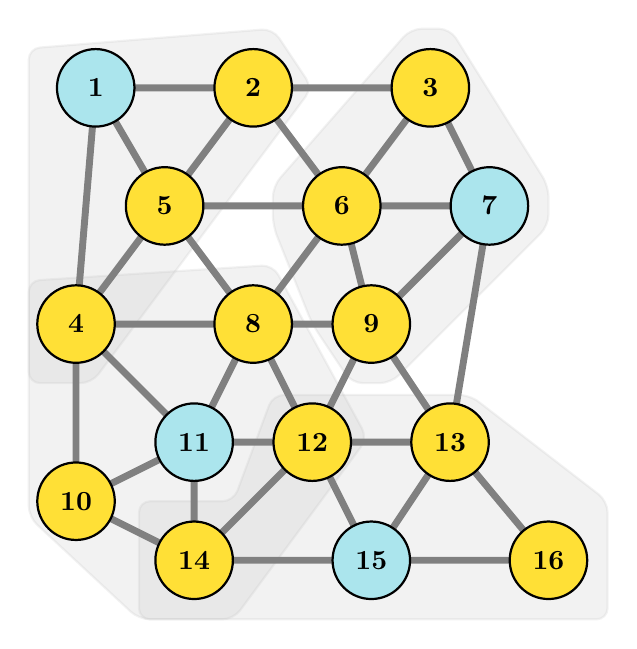
\begin{tikzpicture}[thick,font=\bf]

% Four gray regions
\draw[draw=gray!50,fill=gray!50, opacity=0.2,text opacity=1,thick,rounded corners] (3.5,1.5) -- (4,1.5) -- (4.5,2) -- (6,3.5) -- (6,4) -- (4.75,6) --(4.25,6) -- (2.5,4) -- (2.5,3.5) -- (3,2.25) -- cycle;

\draw[draw=gray!50,fill=gray!50, opacity=0.2,text opacity=1,thick,rounded corners] (0.8,-1.5)-- (6.75,-1.5) -- (6.75,0)-- (5,1.35) -- (2.5,1.35) -- (2,0) -- (0.8,0) -- cycle;

\draw[draw=gray!50,fill=gray!50, opacity=0.2,text opacity=1,thick,rounded corners] (0.8,-1.5)-- (2,-1.5) -- (3.7,0.8) -- (2.5,3)-- (-0.6,2.8) -- (-0.6,-0.2) -- cycle;

\draw[draw=gray!50,fill=gray!50, opacity=0.2,text opacity=1,thick,rounded corners]  (0.2,1.5)-- (3,5.25) -- (2.5,6) -- (-0.6,5.75) -- (-0.6,1.5) -- cycle;

% Edges
\draw[line width=2.5pt,gray] (0,0) coordinate (P10) -- (1.5,-0.75) coordinate (P14) -- (3.75,-0.75) coordinate (P15)-- (4*1.5,-0.75)coordinate (P16) --  (4.75,0.75) coordinate (P13) -- (3,0.75) coordinate (P12) -- (1.5,0.75) coordinate (P11) --(0,2.25) coordinate (P4) -- (2.25,2.25) coordinate (P8) -- (3.75,2.25) coordinate (P9) -- (5.25,3.75) coordinate (P7) -- (4.5,5.25) coordinate (P3) -- (2.25,5.25) coordinate (P2) -- (0.25,5.25) coordinate (P1) -- (1.125,3.75) coordinate (P5) -- (3.375,3.75) coordinate (P6) -- (P7) (P2)--(P5) (P2) -- (P6) (P5) -- (P4) (P5) -- (P8) (P6) -- (P9) (P1)--(P4)--(P10)--(P11) -- (P14) -- (P12) -- (P15) -- (P13) -- (P9) -- (P12) -- (P8) -- (P11) (P8) -- (P6) -- (P3) (P7) -- (P13);


% Nodes
\draw[fill=color1] (P10) circle(14pt) node{10};
\draw[fill=color1] (P14) circle(14pt) node{14};
\draw[fill=color2] (P15) circle(14pt) node{15};
\draw[fill=color1] (P16) circle(14pt) node{16};
\draw[fill=color2] (P11) circle(14pt) node{11};
\draw[fill=color1] (P12) circle(14pt) node{12};
\draw[fill=color1] (P13) circle(14pt) node{13};
\draw[fill=color1] (P4) circle(14pt) node{4};
\draw[fill=color1] (P8) circle(14pt) node{8};
\draw[fill=color1] (P9) circle(14pt) node{9};
\draw[fill=color2] (P7) circle(14pt) node{7};
\draw[fill=color1] (P5) circle(14pt) node{5};
\draw[fill=color1] (P6) circle(14pt) node{6};
\draw[fill=color2] (P1) circle(14pt) node{1};
\draw[fill=color1] (P2) circle(14pt) node{2};
\draw[fill=color1] (P3) circle(14pt) node{3};


\end{tikzpicture}

\end{document}
